\documentclass[12pt,onecolumn]{IEEEtran}

\usepackage{rotating}
\usepackage{tikz}
\usepackage{booktabs}
\usepackage{multicol}
\usepackage{tabularx}
%\usepackage{color}
\usepackage{xcolor}
\usepackage{lastpage}
\usepackage{fancyhdr}
\usepackage{grffile} 
\usepackage{graphicx}
\graphicspath{ {images/} }
\usetikzlibrary{arrows, positioning}
\usepackage{amsmath}
\usepackage{newfloat}
\usepackage{caption}
\usepackage{mathtools,cuted}
\usepackage{lipsum}
\usepackage[final]{pdfpages}
\usepackage{lettrine}
\usepackage{siunitx}
\usepackage{pgfplots}
\usepackage[europeanresistors]{circuitikz}
\usepackage{listings}
\usepackage{verbatim}
\usepackage{pgfgantt}
\usetikzlibrary{arrows}

\lstset{frame=tb,
language=matlab, 
breaklines=true, 
showstringspaces=false, 
columns=flexible, 
numbers=none,
commentstyle=\color{green},
tabsize=3
}

\pgfplotsset{compat=1.14}

\begin{document}
\author{Marion Heimann - 788579 \\ Tristan Kuisis - 812587 \\ Supervisor: Prof Ken Nixon}
\title{ELEN4002 - Preliminary Plan for the Design and Creation of a Wits Analytics and Visualization of Energy Systems Project}
\maketitle
\begin{abstract}
    The main purpose of this document is to outline a project plan for the data analytics and visualization of energy systems across the multiple University of the Witwatersrand (Wits) campuses. The multiple energy meters installed across the properties have been gathering data for a number of years. A web server is to be constructed that is capable of autonomously and repeatedly drawing data from the database. The server will then host a portal that is capable of displaying the data to a user. The web portal will also be used to generate unique visualizations of the data from the sensors.
    This report details the project management aspect of the project to be undertaken.
\end{abstract}
%\begin{IEEEkeywords} 
%Selenium, Visualization, Web Scraping, 
%\end{IEEEkeywords}
\pagestyle{plain}



\section{Introduction} \label{sec:Introduction}
\IEEEPARstart{T}{his} report details the project plan for the data analytics and visualization of energy systems that make up the Wits campuses. 

%There are a number of large energy requirements that Wits has-electricity, water, natural gas, petrol, diesel, as well as a number of other resources which make up smaller fractions of the universities energy usage.
The operation of Wits requires large amounts of energy for various uses. The major resources that are used and can be monitored are- electricity, water, natural gas, petrol, and diesel usage.

This project, firstly makes use of the electricity meters installed throughout the many buildings on the properties. These meters have been providing data for varying amounts of time. Data outages occur occasionally (this will be dealt with). 
The wealth of information that these data loggers provide allow for the creation of a web server which is capable of drawing this data from the database. It will make use of this data to visualize the energy consumption/generation across Wits. The web server will be instrumental in allowing a user to visualize this energy in a multitude of ways.
%The timelines, methods, tools, and a number of other details are discussed throughout this report.


\section{Project Specifications}

\subsection{The Data} \label{sec:TheData}
As discussed above, there are a number of energy meters placed throughout the Wits properties. There are over 300 data loggers that are connected to the current web portal used by the university. 
The web service and data system in place, run by IST \cite{IST}, is based off-campus. %This means that the web service and data is housed on their side. 
All of the data retrieval (from the data loggers) is done through the Wits network and in some cases through a mobile data connection. This element of the project is discussed further down in Sections~\ref{sec:DataGathering}. 

There are two other highly relevant data sets that will be used for the core part of the project. These are: the energy generated by the solar panels installed on top of a number of buildings on the main campus, and the weather at this campus. 
These two data sets will allow for a unique picture to be painted which further enhances the visualization of the system as a whole. 

%Currently, these are the chosen data sets that will be used for the core of the project, however, if time permits, the university holds a wealth of information regarding the location of individuals throughout the university, this is provided with the use of the Integrated Campus Management (ICAM) system which is used for the access control for the university \cite{icam}. 
Currently, these are the chosen data sets that will be used for the core of the project. If time permits, information regarding the location of individuals throughout the university will be used. This is provided with the use of the Integrated Campus Management (ICAM) system which is used for the access control for the university \cite{icam}. The help of individuals from Wits' Business Intelligence Systems (BIS) this information integration will be made possible.
This system is likely to unlock further insights on the universities energy usage and how the movement of individuals affects the energy usage of specific areas. 


\subsection{Back-End} \label{sec:BackEnd}
In order to run the system proposed, a number of operations are required to take place in a selection of programming languages, and all of these should be able to communicate with one another such that the process described by Section~\ref{sec:SystemArchitecture} can take place. 

The back-end can be described by a local web server that is run on the users machine (in this case, the server is run on each ISTPassword' personal computer), and it is important as it allows the simulation of a server that will (ideally) eventually be placed onto a standalone system such that users with internet access will be able to use the system anywhere.
This section is discussed in further detail in Section~\ref{sec:back-end system architecture}.

\subsection{Front-End} \label{sec:FrontEnd}
In order to allow for the visualization of energy, the use of standard front-end web tools will be employed in order to provide the user with interaction. 
The back-end will provide all of the processing requirements, and will manage the data. The front-end communicates with the back-end (server) in order to illustrate the required information.
The three main tools (commonly used in any website), are: Hypertext Markup Language (HTML), Cascading Style Sheets (CSS), and JavaScript. 
These three tools communicate with each other and the server in order to provide the user with the required information when viewed from a web browser. 

It is this part of the system where a multitude of visualization tools are used to gain insights into the data. These tools will be discussed in Section~\ref{sec:ApplicationsAndTools}. \newline

This completes the overall description of how the system is constructed and how it functions in order to get the required functionality.


\section{Scope Statement} \label{sec:ScopeStatement}
There are four sections to the scope for this project, these are: data gathering, back-end system, front-end system, and the ability to use the front-end system to gain insights and visualize the data in multiple ways. %All of these sections together form the scope for the project.

The data gathering system is required to be capable of autonomously, and periodically drawing data from the IST server for all of the data loggers and all of the data that they have attained since installation. There are a few details for this section left for Section~\ref{sec:DataGathering} as the system does not always need to gather in the same way.

The back-end system takes part in the data gathering process, this is why it is important that it functions as required. The back-end deals with all of the data storage, as well as processing of the data in order to send it through to the front-end such that a user can interact with the system. This is used as the system which manages the storage and manipulation of the data which is highly important. 
In order to reduce the work required by the client (front-end), the majority of the presentation work will be done on the server, then once it is ready, sent through to the client. 
There may be cases where client side processing will be used an example of this is Dygraphs. This requires the clients' browser to interact and process information and data\cite{dygraphs}.

The front-end is important for any web application, as this is the interface which allows user interaction.
%, which is where the focus and importance rests. 
The front-end makes use of HTML, CSS, and JavaScript to generate the standard format of the user interface (UI). This configuration is used with a number of other tools in order to have multiple types of data visualization.
The details of the front-end is discussed in Section~\ref{sec:SystemArchitecture}.

Finally, the fourth key part of the scope is that of the data visualization. This will be done with the use of many tools and methods such that insights can be gained from the data. The most important decision for this part of the scope is that the system should be designed such that a greater understanding of the system can be gained. Two examples of this are: verify that the billing from City power matches that which the system measures, and another interesting, possibly engineering test, is to verify how much energy has been saved with the exchange of the old lighting systems to all LED lights throughout campus. 

% Pick a focus: something to attain (see how money works or how new lights changed things)

% Demonstrate concept


\section{Timeline} \label{sec:Timeline}
It is important to illustrate a basic timeline for any project. In this case, the timeline forms a similar order to how the scope is laid out. 
The following list illustrates the important dates for the project, this indicates when certain parts of the project need to be completed. 

\begin{itemize}
    \item 16 July - Project plan due
    \item 16 July - Lab project officially begins
    \item 17 August - Deadline to change project name
    \item 27 August - Staff inspection day
    \item 28 August - Open day
    \item 3 September - Project electronic submission deadline
    \item 13 September - Laboratory project conference - presentations and interviews
\end{itemize}

This indicates that there are approximately six weeks in which the project takes place. 
There is a specific method which the project uses, this is such that minimal functionality can be gained out of the system as soon as possible.
This means that each of the four major sections laid out in the scope will be put together such that the system can be up and running to test out simple functionality. 
This method can be compared to that described in The Pragmatic Programmer, where they illustrate the method of using tracer rounds \cite{pragmatic}, where the use of a full paper design will lead to a successful product, however, in some cases, it may be more beneficial to make use of \textit{tracer rounds} in order to get feedback within a shorter time period and to see the effects of the system quickly. The \textit{tracer rounds} in this project mean a system that has simplistic functionality in each of the components.
The nature of this project is such that the requirements from the \textit{client} can be relatively vague, and this type of project is unique in it's dataset and use case. 
This implies that many of the tools and methods that are used throughout the project will change over time as there are many unknowns throughout the process. 
These unknowns are reduced with the use of prior research and comparing similar systems, however, there will always be a non-zero amount of uncertainty for parts of the project.

%This is why a lot of prior research and testing has taken place before the project begins. 

The following figure, Fig.~\ref{fig:gantt} illustrates a first estimate on how the project timeline will be structured. The gantt chart is set out in working days.

\begin{center}
    \begin{figure}[htb]
        \centering
        \begin{ganttchart}[hgrid, vgrid, inline]{1}{30}
            \gantttitle{Lab Project}{30} \\
            \gantttitlelist{1,...,30}{1} \\
            \ganttbar{A}{1}{3} \\
            \ganttbar{B}{4}{6} \\
            \ganttbar{C}{7}{10} \\
            \ganttbar{D}{11}{12} \\
            \ganttbar{E}{13}{16} \\
            \ganttbar{F}{17}{19} \\
            \ganttbar{G}{20}{20} \\
            \ganttbar{H}{21}{30} \\    
            \ganttbar{I}{1}{30} \\
            \ganttbar{J}{1}{30}    
         %   \ganttlink{elem0}{elem1} 
         %   \ganttlink{elem1}{elem2}
         %   \ganttlink{elem2}{elem3}
         %   \ganttlink{elem3}{elem4}
         %   \ganttlink{elem4}{elem5}
         %   \ganttlink{elem5}{elem6}
         %   \ganttlink{elem6}{elem7}
        \end{ganttchart}
        \caption{Estimate Gantt Chart of Project}
        \label{fig:gantt}
    \end{figure}
\end{center}    
Where: 
\begin{itemize}
    \item A - Data Retrieval
    \item B - Data Storage and Manipulation
    \item C - Back-End Set-up
    \item D - Back-End Link with Data Retrieval System
    \item E - Front-End Design
    \item F - Integration with visualization tools
    \item G - Reassess System
    \item H - Iterative Methodology
    \item I - Documentation
    \item J - System Testing
\end{itemize}

%As it commonly works with gantt charts, there will be tasks which take less time than scheduled, and they can also run over time, this shifts sections of the chart and effects tasks further down the line.
There are a number of tasks which run throughout the entire project (documentation and system testing), this is done as it helps the development process run smoothly and any changes that happen to the system are always tested so that different components in the system are not affected with changes to any other component. This testing helps the interfacing of the different components run smoothly and is discussed further in Section~\ref{sec:DependenciesInterfaces}.

Finally, there is a task called \textit{Iterative Methodology}, this is where the \textit{tracer bullets} methodology is used. All of the tasks before this are set out to get the system up and running so that vulnerabilities and loopholes can be found in the system, and further visualizations can be added to the system. Once the data sets and the system as a whole is functioning, it becomes a matter of working with the data to provide multiple visualizations.

It should be noted that the tasks described in this section have been planned such that they all follow a consecutive order, however, as discussed further down in the report, there are components which can have clearly defined inputs and outputs, this allows for earlier development of components. This means that in some cases, modules can be developed in parallel if required or becomes more productive.

\subsection{Working Times} \label{sec:WorkingTimes}
It has been recommended that the working times for this project should be kept to a standard 08:00 to 17:00 working time, done such that the project can simulate a \textit{project} in industry.
There may be cases where these times will have to be altered such that certain tasks can be completed within scheduled times.

Throughout the project, meetings with the project supervisor, as well as other individuals, will take place; these will be used for consulting purposes and follow up meetings with progress on the project.


\subsection{Milestones and Deliverables} \label{sec:MilestonesAndDeliverables}
There are a number of milestones that are used for the duration of the project, these are mostly made up of the major sections in the scope, and are illustrated below:

\begin{itemize}
    \item Retrieval and Storage of Entire Database
    \item Periodic Retrieval and Storage of Database
    \item Back-End Set-up
    \item Front-End Skeletal Design
    \item Visualizations
    \item Refinement of each stage
\end{itemize}

These are set as the major milestones and deliverables that are currently set out for the project. The nature of the data that is presented by this system affords a highly important resource for major stakeholders in the Wits community.
% A number of stakeholders have been contacted and asked for their input on the system, meetings will take place with these people throughout the project.
The input from these stakeholders can guide the later stages of the project as it will be their ideas/questions which determine what the major visualizations and information should be.% inferable from the data.
This input allows for these later milestones and deliverables to be more defined.
% Meetings with stakeholders + implement their suggestions


\section{Risks} \label{sec:Risks}
Risks appear in all projects, these risks need to be: assessed and analysed, evaluated, and in some cases, treated and responded to.
The risk management process and methods will be applied to these risks such that the success of the project is not compromised.
Some of the risks posed by this project are unavoidable and will be dealt with on a case by case basis.
%Other risks can have contingency plans in place. 
A list of possible risks are discussed in the subsections to follow.


\subsection{Data Outages} \label{sec:DataOutages}
Data loggers can be damaged, data corruption occurs, or data is lost. This can happen for a number of reasons, and results in outages of the data.
There are a number of ways in which the system can be made to estimate the missing data points, however, this will never represent the actual data that was present in the first case.

The way in which the data loggers are installed throughout the university is such that many were installed at different times. 
This means that, as one looks further back into the past, the picture painted by the data becomes less indicative of the energy usage across most of the university. 

In some cases, it is can be useful to visualize just where the data is missing, rather than estimating what the data was in that outage.
This implies that the project can make use of this missing data to its advantage. There are a number of tools that allow one to make use of this fact \cite{missingdata1,missingdata2}.

This fact about the system can end up requiring a large amount of work, which can mean manipulating the data to suit the users needs.

A second important point to note about the data outages is where the data is coming from, this is introduced in the following subsection.

\subsection{Web Scraping Dependencies} \label{sec:WebScrapingDependencies}
A major portion of the project relies on the data relayed by IST. IST are in control of the database, and currently, the only method to access this data is through the web portal. Gathering the data from this system has posed some potential challenges which have currently been overcome with the use of web scraping tools. 
These tools simulate user interaction on the website in order to download the data from the website in chunks. The web scraping tool is manipulated such that it enters the information and selects the buttons that a user would when interacting with the website. 
This poses a risk for gathering data if the website is changed, resulting in the scripts no longer functioning as they required.
The use of this web scraping tool is employed for this first section of the project as direct access to the database has not yet been granted.
The risk that this poses is unlikely to heavily impact the project as the chances of the website being altered within the allotted time for the project is low.

The solar panels provide a non-negligible amount of energy to the campus, and this system provides users with energy generation data. The web scraping tools will also be used to draw the relevant data. This method of drawing the data will also have the same risk posed as it can stop functioning with changes to the site structure.

Included in this section is that of the security and validity of the data provided from this system. It is assumed that the data housed by IST will be safe and secure for the duration of the project and for the continued use of the system.
%The access to this system has been granted to the student group for the duration of the project and it is assumed that access to the site will be granted for the duration.
During the research of the web scraping tools in the July holidays, there were periods where the site was down for maintenance, and there were also periods where it had reduced performance, this resulted in slow page load times. Fortunately this happened before the official start of the project, however, if it does occur during the project, it can have an impact on the projects timeline.

\subsection{Intellectual Property and Ethics} \label{sec:IntellectualPropertyEthics}

The university is a public research institution, which means that the information generated is available to the public. The information gathered from this system has not been released to the public before this point.  As energy costs are publicly available, this project has a large responsibility for how the data is handled. The system currently in place is used as an accounts verifier among other uses. This means that the data on the system should not be tampered with, corrupted, or lost.  The relevant stakeholders will assist in the correct way to acquire this data safely. During the web scraping testing, it appears as if the security of the system is not as it should be as the users have direct read and write access to the data.
%This implies that the handling of this system should be handled with care.


% Table for risks
\begin{table}[!t]
% increase table row spacing, adjust to taste
\renewcommand{\arraystretch}{1.3}
%if using array.sty, it might be a good idea to tweak the value of
%\extrarowheight as needed to properly center the text within the cells
\caption{Risks}
\label{tab:risks}
\centering
% Some packages, such as MDW tools, offer better commands for making tables
% than the plain LaTeX2e tabular which is used here.
\begin{tabular}{p{50mm}p{15mm}p{15mm}p{80mm}}
\hline
Risk & Risk Level Likelihood (1-10) & Risk Impact (1-10) & Comments \\
\hline
IST System Down & 4 & 8 & No access to system means no data access \\
IST System Crash & 2 & 9 & Loss of data implies loss of historic data \\
IST System Change & 6 & 5 & Lose time because it means editing of web scraping system \\
Project Data Loss (damaged computer) & 3 & 1 & The codebase and documentation is stored on the github repository \\
Team's inability & 2 & 7 & If required, assistance is available \\
Intellectual Property/Plagiarism & 2 & 9 &  \\
Internet Access Loss & 5 & 2 & Wits internet can be intermittent which reduces productivity \\
Lack of Weather Data & 3 & 5 & Decreased ability to visualize impact of weather due to reduced sensor fusion \\
Budget Risk & 1 & 3 & Currently there is no forseen expenses \\
Miscommunication & 4 & 6 & Time wasted \\
Changes in Tools (leading to malfunctioning system) & 3 & 5 & Loss of time in getting the system working again \\
Missing Data & 8 & 5 & Inventive ways will need to be used to manage this quirk of the data \\
\hline
\end{tabular}
\end{table}

\subsection{Licensing} \label{sec:Licensing}
This project is likely to make use of a large number of programming languages and tools in order to get the functionality required. Consequently, the licenses of these tools are considered for use. At this stage of the project, it is not planned for the program to be sold as a product or make any revenue.
However, in such a case that the project is successful, it will be easier for future work to take place if the tools used have GPL or MIT licenses. This reduces the future work to change out the tools which required licenses. Some simple guidelines are used for choosing tools throughout the project; GPL, MIT, or similar take preference \cite{yegor}.


\section{System Architecture} \label{sec:SystemArchitecture}

This section discusses the general structure of the components and how they interact.
Illustrated in Fig.~\ref{fig:dataloggers} represents the data loggers and their connection to the relevant buildings, transformers, and systems- each of which is then connected to the IST system.

\begin{center}
    \begin{figure}[htb]
        \centering
        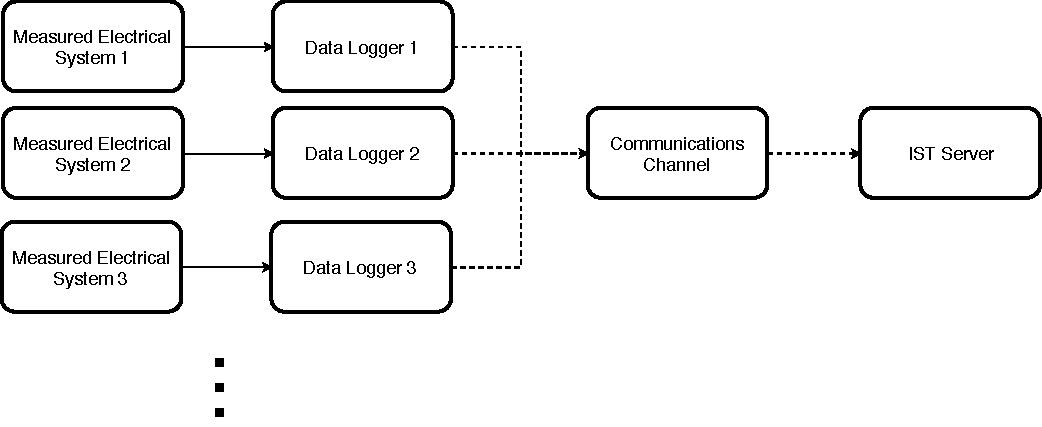
\includegraphics[width=0.8\textwidth]{Data Logger.pdf}
        \caption{Data Loggers and their Connection to the IST Server}
        \label{fig:dataloggers}
    \end{figure}
\end{center}
In the figure, the devices measured can be from multiple different sources. They can be connected to main transformers, or to individual buildings. The managing of all of these buildings and how the systems are interconnected will require some work as there will be cases where one data logger will be measuring a main incomer, and several other data loggers will make up the buildings that are supplied by that incomer.
Once the data has been drawn from the data loggers, it will be a matter of piecing together the sensors so the system can be represented correctly.
The line connecting data loggers to their relevant systems are direct connections via the sensors. The data loggers are then connected to the communications channel via differing methods. Some of the data loggers are connected to the server via the Wits network, and some via 3G or other communications media. The methods by which the data loggers are connected to the system are not of importance to this project and are not investigated.
%, unless it proves to be beneficial to get an idea of which method of communication results in higher data outages.

The IST server, as discussed above draws data from the meters every thirty minutes. This is then stored on the IST database for use on the ecWin web portal.

%\newline
The next section is that of the back-end, it becomes pertinent to illustrate the two together as they work together to create the system. 

\begin{itemize}
    \item Back-End
    \begin{itemize}
        \item Node.js
        \item Python
        \item Python Flask
        \item Python Beautiful Soup
        \item Python Requests
        \item Selenium
        \item Tableau
        \item SlashDB
    \end{itemize}
    \item Front-End
    \begin{itemize}
        \item HTML
        \item CSS
        \item JavaScript
        \item D3.js
        \item Dygraphs
        \item Google Maps
    \end{itemize}
\end{itemize}

\subsection{The Back-End} \label{sec:back-end system architecture}
The back-end will be run on local machines so the system can be hosted locally while development is under way.
The local server is run by making use of Python's Flask package, working hand in hand with Node.js to manage the different languages and tasks required.

Python will handle the majority of the calculations and data manipulation for the system. There are multiple Python packages which are used, and are listed below:
\newline
Python Beautiful Soup: Web scraping tool that draws data from the HTML pages required.

Python Requests: Another web scraping tool which allows the system to make HTTP requests to specific web pages and gather data from those sites. 

Python Selenium: Selenium is a package that is available from the Python database, it is used as a higher level of web scraping, such that a script is capable of further and more advanced web scraping capabilities. This tool is capable of interacting with the JavaScript layer of the web page, where the other tools fall short. The use of this package is highly useful for the ecWin website as well as the solar panel web portals as they make use of this system where no information is found within the HTML page.

The next three tools: D3.js, Dygraphs, and Tableau are used for the visualizing of specific parts of the data. This not a final list of tools to be used, however, it is believed that the first two tools will feature heavily in the final system.

It is important to consider what format the data will be stored. Commonly, standard relational databases are used for managing some kinds of datasets. However, it must be noted that Dygraphs is designed to work with a number of database types \cite{dygraphs_data}. The database that is used should be chosen based on a number of factors: performance, size, ease of use, visualization tool requirements, etc \cite{database}. SlashDB is seen to be a commonly used database with D3.js, however, the implementation of databases is not limited to this.
The database is important as this is the interface between the data, and the tools used by the system. It may be the case that one database type does not have to be the only one implemented; there may be multiple database formats used for the different tools.

\subsection{The Front-End} \label{sec:TheFrontEnd}
The front-end has been discussed in some detail above, however it is important to note that in most cases the front-end will be designed such that the majority of the work will be done by the server side. A number of tools used do, however, require some processing on the client side. The processing on the client side will come about because of the data visualization tools such as Dygraphs and D3.js. 

Google Maps is an interesting addition to the front-end, as an attempt to show energy usage overlaid on a map can provide a different perspective on the system.

This is likely to be a small selection of the tools that the project will eventually use, however, these will be capable of undertaking the majority of the visualization needs.


\subsection{Dependencies and Interfaces} \label{sec:DependenciesInterfaces}
The aspect of interfaces was discussed above, however, this forms an integral part of the project as there are many components which are required to work together for the system to function.
Every component should be designed such that its inputs and outputs are clearly defined such that it can work seamlessly with the surrounding components. 
An example of this is that of the web scraping tool- it is required to gather csv files from a website, it expects these csv files to be of a specific format, it is then expected that this system place these files in a folder with a name that is standardised with the next component in the system.
This allows for efficient modularity within the system and if there are cases where specific components need to be changed, it does not affect other components within the system.
The dependencies and interface requirements of all of these components is specified in the documentation and comments of the code of the component. This allows for easy modification down the line. 

The other important consideration for the system is dependencies of the tools required for the system to function. There will be a multitude of tools used throughout all with different requirements and settings so that they can be used effectively. These dependencies will also form part of the documentation of the system for future use.


% \subsection{Website/Portal Architecture} \label{sec:WebsiteArchitecture}

% \begin{enumerate}
% \item Prepare for the activity of sitemapping
% \item Brainstorm the types of content
% \item Define primary navigation
% \item Flesh out second and third level structure and content
% \item Don’t forget about utility pages
% \item Create notes and high-level specifications for each page
% \item Designate the type of design template
% \item Iterate. Iterate. Iterate.
% \end{enumerate}

% Maps which illustrate how one navigates through the website. 

\section{Resources} \label{sec:Resources}
The nature of this project is such that open source and freely available tools will be used to create the system. This implies that a budget will not be required for the project. There is a set budget which is allocated for each project and it is unlikely that any of this budget will be used for the project.
The tools which potentially require licenses (eg. Matlab) will be provided by the school, however, it is unlikely that these tools will be used at this point as they do not currently have a use in the project. 

The project is heavily based on the use of software tools and machines on which to develop the system. The ISTPassword will make use of their personal machines to do this. There may be cases where a more powerful machine may need to be used, in this case the machines in the D-lab will be utilised. 

The major cost in this system has already been covered, this is the cost of the data loggers and the servers provided by IST. This has been put in place over the last few years by the university.





\section{Applications and Tools} \label{sec:ApplicationsAndTools}

This section details the auxiliary tools used during the development of the system.
The first of these tools, the operating system, is Windows 10, chosen as this operating system is already installed on the ISTPassword machines before the project started. % and also from a familiarity point of view. 
Ideally, the system should eventually be placed onto a server, which will likely be running a distribution of Linux, so considerations should be made for the structure of the system such that porting the system will be a simple affair. 
The tools that are discussed in this report are useful in that they can easily be used on both operating systems with minimal change to the overarching system. 
During development, however, the design should be such that the system can run on as many different machines while requiring little to no editing of the code base.

The system will require a large amount of software writing, as such the use of Visual Studio Code will be used for the majority of the editing. This is chosen as it is open source, and has a large third party extensions database which makes the development process easier. 

A version control software is used throughout the development of the project. Since the bidding stage, a git repository has been used that the two ISTPassword can work with. The git repository is currently hosted on gitHub using a private repository.

This system allows for convenient and safe work on the project to take place. The repository allows the two users to work remotely while developing different aspects of the project at the same time. 




\section{Development Approach} \label{sec:Development Approach}
%This project is undertaken by a project team of two people, this implies that some of the development methods like agile, waterfall, scrum *** cannot be used as they require much larger teams in order to work effectively. 
%*** Talk some more about this \cite{}.

The programming methodology discussed in \textit{The Pragmatic Programmer} is made use of throughout the project, this is: work iteratively, make small changes to the system and re-evaluate. 

In any software project, documentation plays a role. It needs to be present in some form. There are many different ways of documenting a project. One commonly used way is to create and manage a Wiki; this means that all of the documentation for the project can be found in one place \cite{documentationpost}. 
A second popular method is to make use of markdown files throughout the system. This forms part of the repository and can be found alongside the code.

Make sure that as code is written, it is commented and documentation is made for that section. Documentation is highly important for the success of the project because it should be able to be used by future teams. % who work on the system and further its capabilities. 
Up to this point, markdown files have been used to document meetings, notes, ideas, etc. and will continue to be used for the time being. The use of a Wiki, or other similar documentation structure may be considered at a later stage during the project. It might be worth investigating the use of GitHub Wiki which will work hand in hand with the currently used GitHub repository \cite{githubwiki}.
These markdown files form an instruction manual for the different parts of the system.


% **** How to do documentation properly in this system with so many programming languages

Testing of the system is done throughout the development process, this is such that each and every component can be automatically verified that it does what it should do. 
The interface of each component in the project will be tested using this testing procedure. 

%Unit testing forms large parts of any software development process. 
%Unit testing is commonly used to test the functionality of specific functions of code and is highly useful in object-oriented systems. Unit testing forms a part of the testing processes.
There are multiple types of testing which may become useful for the system to implement: unit testing, integration testing, component interface testing, system testing, and operational acceptance testing \cite{swebok}.
The package, Selenium, becomes highly relevant when testing out the front-end as it emulates the process that would happen for when a user is interacting with the system. This tool has been used extensively by Dropbox for their product line, indicating a reliability in this type of testing for websites \cite{dropbox}.

%In this case unit testing can take the form of testing out the server in its executions for drawing data, managing data and working with the front end.



\bibliography{IEEEabrv,References}
\bibliographystyle{IEEEtran}

\appendix
%\section{Server} \label{sec:Server}
\section*{Data Gathering} \label{sec:DataGathering}
%weather data

The system has a collection schedule set at thirty minutes, this means that each of the data loggers is sent a request, and the data is the sent to the IST servers, where it is stored in their database \cite{datasite}.


IST host a web service which allows customers to view the relevant information from these data loggers. 
The web portal allows the user to view a range of details about the system, the homepage of the system is illustrated in Fig.~\ref{fig:ecwin}.

\begin{center}
    \begin{figure}[htb]
        \centering
        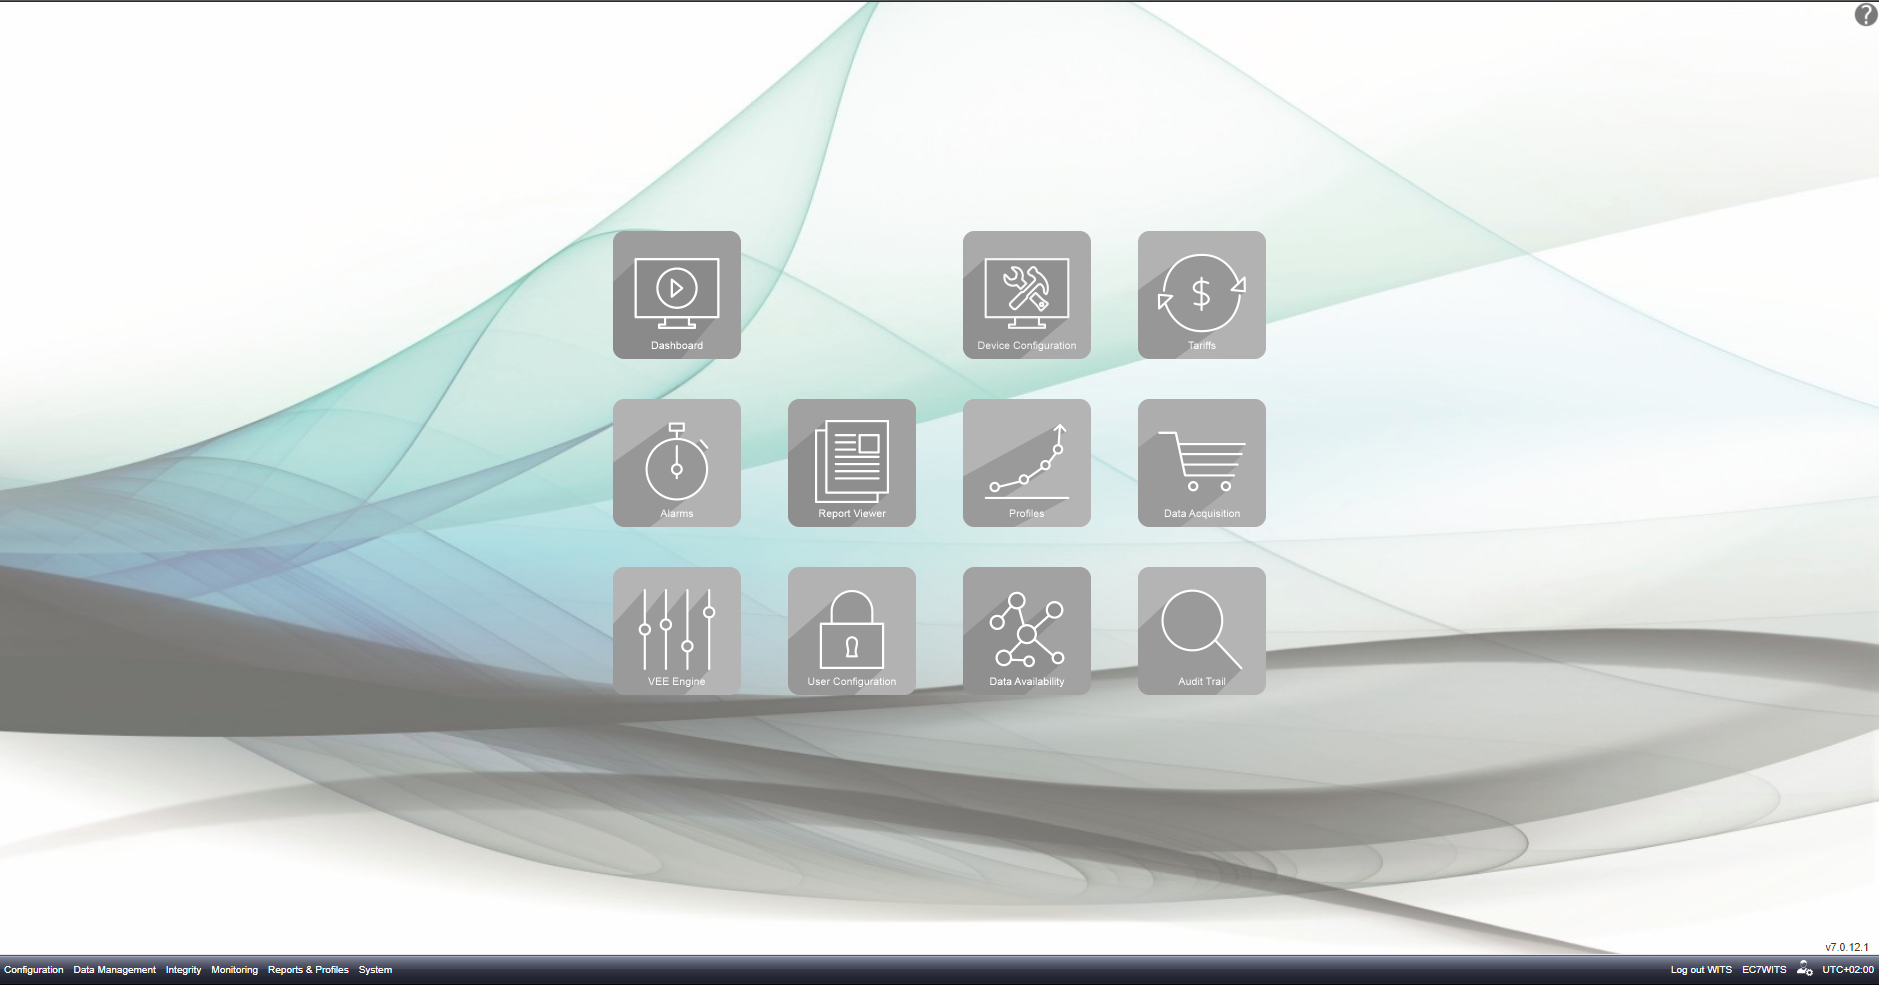
\includegraphics[width=0.8\textwidth]{ecwin.png}
        \caption{ecWIN Web Portal}
        \label{fig:ecwin}
    \end{figure}
\end{center}

This is the web portal that is to be used to gather the data from, this can be done by navigating to two different sections of the system: through the data editor section, and through the reports section. Both of these are, however, limited in their functionality. It must be noted that access to the IST database directly has not been granted as of writing this report, this is why the following methods have been utilised.

The data editor has a major shortfall in that one can only view the data loggers' data in small intervals, this means that when gathering the data for the specific meters, the system will have to download multiple files and then stitch them together to get complete representation of the data from that meter.

The reports section allows the user to view the data with no limits on the date range, however, when one selects the option to export the data, an error occurs (illustrated in Fig.~\ref{fig:ecwinerror}). 

\begin{center}
    \begin{figure}[htb]
        \centering
        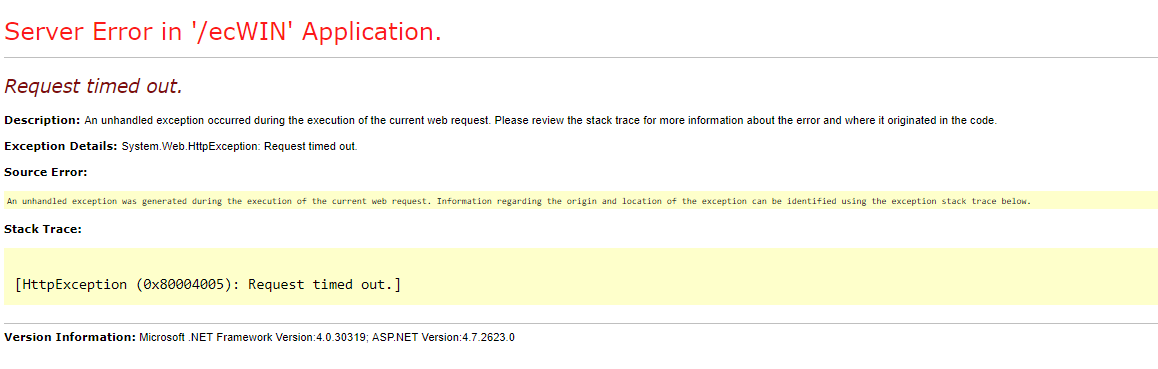
\includegraphics[width=0.8\textwidth]{ecwinerror.png}
        \caption{ecWIN Data Export Error}
        \label{fig:ecwinerror}
    \end{figure}
\end{center}

Thus, the choice of gathering the data from the data editor is chosen, and the method of gathering this data is further discussed in section~\ref{sec:DataGathering}.

As alluded to earlier in the report, the system will not always draw data going back to the installation of each datalogger. Once the system has stored the entire dataset, it only needs to download the latest entries in order to keep updated, this reduces the load on the server and the time taken to update to the latest entries. 
The system should also have the ability to verify the data that it has within its database, as there can be changes to the IST database once the data has already been extracted.
% Firstly to download all of the data going back... Then once this has happened, keep downloading the data periodically.
% A system must be in place so that the system can check up on the validity of the data that it has downloaded and compare it to the data on the server. 

%\section{Data Conversion} \label{sec:DataConversion}

%\section{Data Manipulation} \label{sec:DataManipulation}

%\section{Accessibility} \label{sec:Accessibility}

%\section{Insights} \label{sec:Insights}





% \newpage
%\onecolumn
%\appendix


\end{document}